
\documentclass[a4paper, oneside, 11pt]{report}
\usepackage{epsfig,pifont,float,multirow,amsmath,amssymb}
\newcommand{\mc}{\multicolumn{1}{c|}}
\newcommand{\mb}{\mathbf}
\newcommand{\mi}{\mathit}
\newcommand{\oa}{\overrightarrow}
\newcommand{\bs}{\boldsymbol}
\newcommand{\ra}{\rightarrow}
\newcommand{\la}{\leftarrow}
\usepackage{algorithm}
\usepackage{algorithmic}
\topmargin = 0pt
\voffset = -80pt
\oddsidemargin = 15pt
\textwidth = 425pt
\textheight = 750pt

\begin{document}

\begin{titlepage}
\begin{center}
\rule{12cm}{1mm} \\
\vspace{1cm}
{\large  CMP-6048A Advanced Programming}
\vspace{7.5cm}
\\{\Large Project Report - 15 December 2021}
\vspace{1.5cm}
\\{\LARGE Maths Interpreter Software}
\vspace{1.0cm}
\\{\Large Group members: \\ James Mason and Nia Preston}
\vspace{10.0cm}
\\{\large School of Computing Sciences, University of East Anglia}
\\ \rule{12cm}{0.5mm}
\\ \hspace{8.5cm} {\large Version 1.0}
\end{center}
\end{titlepage}


\setcounter{page}{1}
%\pagenumbering{roman}
%\newpage


\begin{abstract}
An abstract is a brief summary (maximum 250 words) of your entire project. It should cover your objectives, your methodology used, how you implemented the methodology for your specific results and what your final results are, your final outcome or deliverable and conclusion. You do not cover literature reviews or background in an abstract nor should you use abbreviations or acronyms. In the remainder of the report the chapter titles are suggestions and can be changed (or you can add more chapters if you wish to do so). This template is designed to help you write a clear report but you are welcome to modify it (at your peril ...). Finally, a guideline in size is approximately 3,500 words (not including abstract, captions and references) but no real limit on figures, tables, etc.
\end{abstract}

\chapter{Introduction}
\label{chap:intro}


\section{Project statement}
The purpose of this project is to create a piece of software that is an interpreter for mathematical functions. It will run both as an interactive prompt and a utility to interpret and execute pre-written files.
It will additionally provide the ability to visualise mathematical functions such as on a graph.

\section{MoSCoW}
\subsection{Musts}

These elements largely comprise the minimum functional requirements of the program and are as such the most neceassary items.
\begin{itemize}
	\item Expressions
	\item Statements
	\item Commands
	\item Custom syntax using a custom lexer and parser
\end{itemize}

\subsection{Shoulds}

\begin{itemize}
	\item Function visualisation
	\item Intuitive UI
	\item Flexible and scalable architecture
	\item Parallel processing of intensive operations
	\item Simple trigonometric functions
\end{itemize}

\subsection{Coulds}
\begin{itemize}
	\item Interactive visualisations
	\item Zero-crossings finder
	\item Differentiation and integration of functions
	\item Simple equation solver (for example finding a variable)
\end{itemize}

\subsection{Won'ts}
\begin{itemize}
	\item Imaginary numbers
	\item 3D function graphing
	\item Multi-variable equation solver (beyond simple simultaneous equations)
\end{itemize}

\section{Report structure}
Breifly describe what you will cover in the remainder of the report, chapter by chapter.

\chapter{Background}

Depending on the nature of the project, this chapter may cover a literature, resource and/or (software) product review. For a literature review you will consult journal or conference papers outlining methodologies that you may (or may not) use but which are definitely relevant to your particular problem. Resource and/or product information will typcially be substantiated through internet links. 
You may use different sections if different subareas are part of your problem statement and/or solution. 
Since this chapter covers background resources, you should also update the corresponding bib file referred to in the bottom of this document and here it is called References.bib.
You cite references like this: Taylor et al. \cite{Taylor:2007} investigated non-linear FEA on the GPU. Morton \cite{Morton:1966} developed a file sequencing method in 1966. A website on OpenCL can be found here \cite{Soos:2012}. Etc.

\chapter{Methodology}\label{MethLab}

Describe here various methods that will be used in your project. Use different sections for distinctly different subjects and use subsections for specific details on the same subject. Only use subsubsections or paragraphs (which are not numbered) if you believe this is really necessary. Since implementation will happen in sprints, this section may need several updates with parts being added and deleted across the project.

\section{Method 1}
\subsection{Method 1 specific detail 1}
In case you need maths, here is an example to write an equation:
\begin{equation}\label{weak_form}
\int_{\Omega_0} \delta u \frac{\partial \mathbf{P}}{\partial X}d\Omega_0 + \int_{\Omega_0} \delta u \mathbf{b} d\Omega_0 + \int_{\Omega_0} \delta u  \rho_0\mathbf{\ddot u} d\Omega_0 = 0
\end{equation}
And here we show how to write a matrix equation:
\begin{equation}\label{Jacobian}
 \mathbf{X}  \frac{\partial N}{\partial e_c} =  \left[  \begin{array}{cccc} x_1 & x_2 & x_3 & x_4 \\  y_1 & y_2 & y_3 & y_4 \\  z_1 & z_2 & z_3 & z_4 \end{array} \right] \left[  \begin{array}{ccc} 1 & 0 & 0 \\ 0 & 1 & 0 \\ 0 & 0& 1 \\  -1 & -1 &  -1  \end{array} \right] 
\end{equation}


\subsection{Method 1 specific detail 2}
blablabla

\paragraph blablabla

\section{Method 2}

\subsection{Method 2 specific detail 1}

\section{Etc.}

\subsection{Etc.}

\chapter{Implementation}\label{Impl}

In this chapter you cover the actual implementation of your project. Implementation will be done in sprints so you may wish to use different sub-sections for each sprint and then dedicate a section to your final deliverable. Section \ref{Figures} with figures  should not remain in the final report.

\section{Early sprints}
\subsection{Sprint 1}

\subsection{Sprint n}

\section{Final implementation}

\section{Figures, tables, etc.}
\label{Figures}

The purpose of this section is to just show you how to integrate figures, tables, etc.\ and should disappear in the final report. Figures and tables should be distributed across the document wherever they are needed but you should use an appendix if they are many figures/tables of the same kind. Fig.\ \ref{Pelvis_BVH} shows a bony pelvis.

\begin{figure}[htb]
%\begin{center}
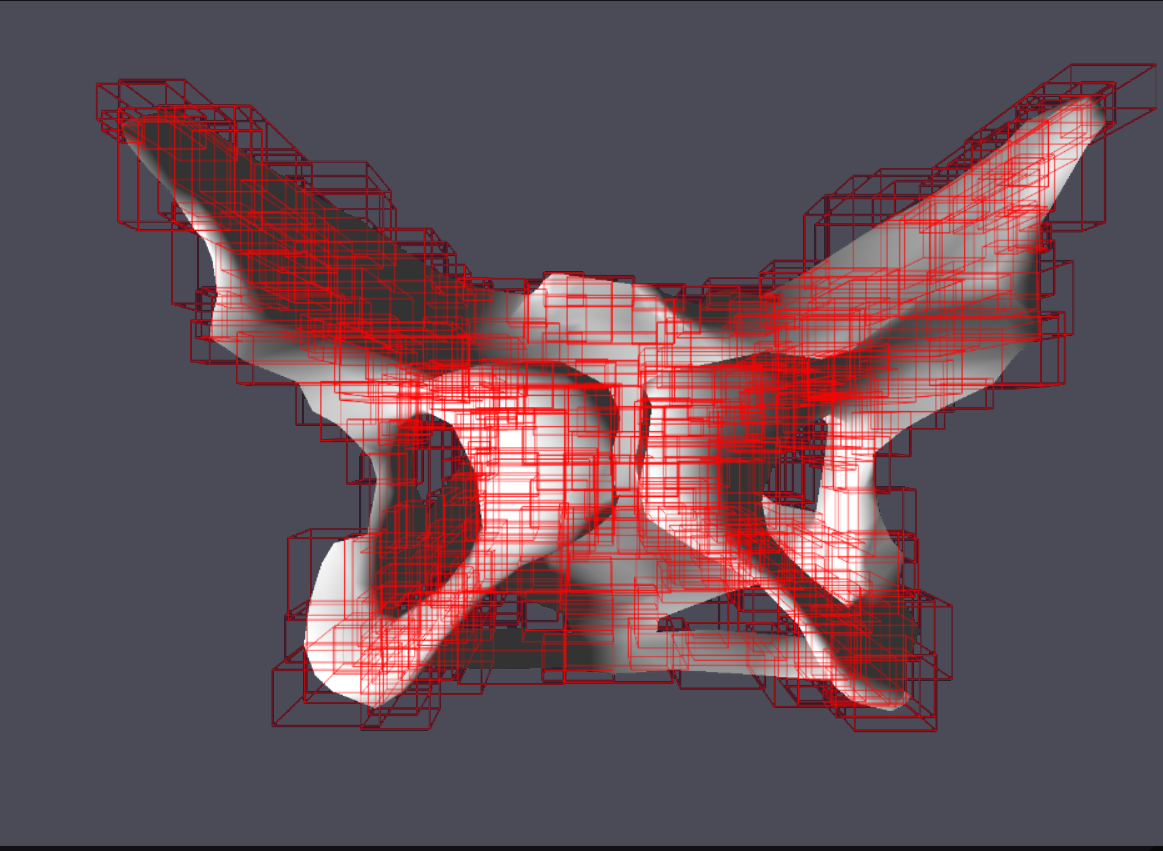
\includegraphics[width=1.0 \columnwidth]{pelvis_octree.png}
\caption{The bony pelvis model with octree based AABBs (Axis Aligned Bounding Boxes).}
\label{Pelvis_BVH}
%\end{center}
\end{figure}

Fig.\ \ref{class} shows a UML class diagram (class, sequence and state diagrams are the most frequently used UML diagrams):

\begin{figure}[htb]
%\begin{center}
\includegraphics[width=1.0 \columnwidth]{class.png}
\caption{A UML class diagram.}
\label{class}
%\end{center}
\end{figure}

Algorithms can be either used in this chapter or alternatively in Chapter \ref{MethLab} if it is a more generic algorithm:

\begin{algorithm}[th]
\caption{ The projection based contact method algorithm }
\begin{algorithmic}[1]
\STATE Retrieve current node displacement $u$
\\ \texttt{float3 u = m\_U\_new[nodeIndex].xyz;}
\STATE Retrieve constraint plane equation
\\ \texttt{float4 plane = m\_constraintMagnitude[nodeIndex];}
\STATE Calculate dot product with plane normal
\\ \texttt{float d = dot(u, plane.xyz);}
\STATE Find node penetration into the plane's negative half-space
\\ \texttt{float penetration = plane.w - d;}
\IF {penetration is greater than zero}
	\STATE Find projection onto the plane surface
	
	\texttt{float3 proj = u + plane.xyz * penetration;}
	\STATE Prescribe new nodal position to be on the surface
	
	\texttt{m\_U\_new[nodeIndex] = (float4)(proj, 0.0f);}
\ENDIF
\end{algorithmic}
\end{algorithm}

Tables such as Table \ref{Res01} can also be useful here or in Chapter \ref{MethLab}.

\begin{table}[h]
\caption[]{Original diameters and diametral strains as reported by
  Sorbe and Dahlgren \cite{Sorbe:1983} (columns 1-2), from a previous 
  experiment by Lapeer and Prager and reported in \cite{Lapeer:2001}
  (columns 3-4), and from the current experiment (columns 5-6).}
\begin{center}
\begin{tabular}{|l|c|c||c|c||c|c|}\hline
& \multicolumn{2}{c||}{S-D} & \multicolumn{2}{c||}{L-P old} & \multicolumn{2}{c|}{L-P new} \\ \hline
Diameter & length & strain & length & strain & length & strain \\ \hline
$\mi{MaVD}$ & 140.5 & +1.90 & 129.3 & +0.30 & 129.3 & +1.43 \\
$\mi{OrOD}$ & 131.4 & +0.10 &   -   &  -    & 119.9 & +1.85 \\
$\mi{OrVD}$ & 126.9 & +2.20 & 119.3 & +0.25 & 119.3 & +1.24 \\
$\mi{OFD}$  & 134.0 & +0.40 &  -    &   -   & 119.7 & +1.82 \\ 
$\mi{SOFD}$ &  -    &   -   &  -    &   -   & 113.2 & -0.85 \\
$\mi{SOBD}$ & 117.1 & -1.70 &  88.7 & -1.07 &  88.7 & -2.52 \\
$\mi{BPD}$  & 105.0 &  0.00 &  89.7 & -0.21 &  89.7 & -0.83 \\ \hline
\end{tabular}
\label{Res01}
\end{center}
\end{table}

Note that code snippets or lists of crucial programming code or large UML diagrams should go in the Appendix/Appendices.


\chapter{Testing}

Describe various experiments you designed to test your software product. This could be subdivided to be in line with the Sprints in Chapter \ref{Impl}. In case you have protocols which cover various pages, please put them in an appendix (e.g. Appendix A) instead.

\chapter{Discussion, conclusion and future work}

Briefly discuss and conclude your achievements and put them in perspective with the MoSCoW analysis you did early on. Be honest by declaring for example `S' categorised objectives which did not make it to the final deliverable rather than reversely modifying your MoSCoW in Chapter \ref{chap:intro}! Also discuss future developments and how you see the deliverable improving if more time could be spent. Note that this section should not be used as a medium to vent frustrations on whatever did not work out (pandemic, group partners, etc.) as there are other means for this (labs, e-mail MO, ...) that should be used well before any such problems become an issue.


\bibliographystyle{unsrt}
\bibliography{References}

\chapter*{Contributions}

State here the \% contribution to the project of each individual member of the group and describe in brief what each member has done (if this corresponds to particular sections in the report then please specify these).

\chapter*{Appendix A}

Put in tables of data or protocols (e.g. for testing) or code listings or UML diagrams which may take up several pages and do not sit well in the main body text.

\end{document}

